\section{Results}
\label{sec:results}

\begin{figure}[t]
\centering
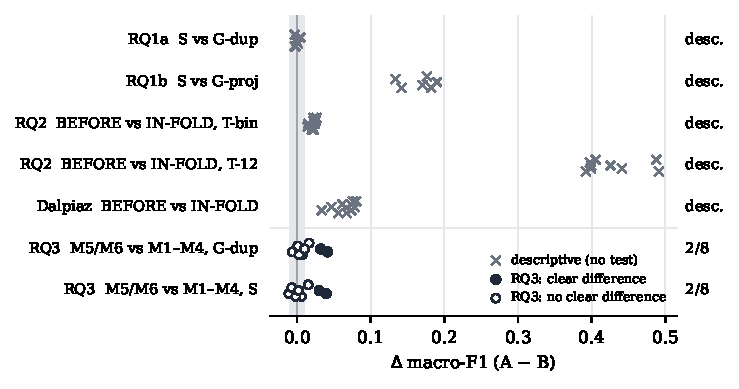
\includegraphics[width=\columnwidth]{figures/summary_deltas.pdf}
\caption{Mean difference in macro-F1 for every planned comparison (one marker per model or model$\times$oversampler). Crosses: comparisons across protocols or oversampling conditions, reported descriptively (difference of means; different test folds). Circles: RQ3, tested on the same splits; filled = clear difference ($|\Delta| \geq 0.01$ and Holm-adjusted $p < 0.05$), hollow = no clear difference. Grey band: $|\Delta| < 0.01$. Right: clear differences per tested family.}
\label{fig:summary}
\Description{Dot plot of mean macro-F1 differences for every planned comparison, grouped by research question, with a grey band marking differences below 0.01.}
\end{figure}

Fig.~\ref{fig:summary} shows all planned comparisons. For RQ1, RQ2 and the replication the test folds differ, so these comparisons are differences of means (Section~\ref{sec:method}). Two of them are large compared with the variation between folds: S vs.\ G-proj and BEFORE vs.\ IN-FOLD on the 12-class task. In RQ3, where models share the same splits, 2 of 8 comparisons show a clear difference under G-dup and under S. The dummy classifier M0 scored a macro-F1 of about 0.35 under every protocol.

\subsection{RQ1: Duplicate- and project-grouped evaluation}
\begin{table*}[t]
\centering
\caption{RQ1: macro-F1 under stratified CV (S), duplicate-grouped CV (G-dup) and project-grouped CV (G-proj) on PROMISE\_exp, T-bin, no oversampling. $\Delta$ = S $-$ grouped (difference of means). Descriptive only: the protocols use different test folds, so no paired test is applied (mean $\pm$ SD over 5 seeds $\times$ 5 folds).}
\label{tab:rq1}
\small
\setlength{\tabcolsep}{4pt}
\begin{tabular}{lrrrrr}
\toprule
& \multicolumn{3}{c}{Macro-F1} & \multicolumn{2}{c}{$\Delta$} \\
\cmidrule(lr){2-4}\cmidrule(lr){5-6}
Model & S & G-dup & G-proj & S $-$ G-dup & S $-$ G-proj \\
\midrule
M0 & $0.351 \pm 0.000$ & $0.351 \pm 0.000$ & $0.352 \pm 0.008$ & -- & -- \\
M1 & $0.876 \pm 0.020$ & $0.878 \pm 0.025$ & $0.694 \pm 0.094$ & $-0.002$ & $+0.182$ \\
M2 & $0.893 \pm 0.019$ & $0.891 \pm 0.018$ & $0.722 \pm 0.061$ & $+0.001$ & $+0.171$ \\
M3 & $0.851 \pm 0.031$ & $0.853 \pm 0.022$ & $0.661 \pm 0.113$ & $-0.001$ & $+0.190$ \\
M4 & $0.889 \pm 0.019$ & $0.884 \pm 0.025$ & $0.755 \pm 0.055$ & $+0.005$ & $+0.134$ \\
M5 & $0.882 \pm 0.023$ & $0.885 \pm 0.019$ & $0.705 \pm 0.083$ & $-0.003$ & $+0.176$ \\
M6 & $0.891 \pm 0.018$ & $0.894 \pm 0.019$ & $0.749 \pm 0.052$ & $-0.003$ & $+0.142$ \\
\bottomrule
\end{tabular}
\end{table*}


\textbf{S vs.\ G-dup.} Grouping duplicates left the estimates almost unchanged (Table~\ref{tab:rq1}). $\Delta$ ranged from $-0.003$ to $+0.005$. That is below the 0.01 threshold for every model and far below the fold standard deviation (0.018 to 0.031 under S, 0.018 to 0.025 under G-dup). Kendall's $\tau$ between the two rankings is 0.733 (Table~\ref{tab:kendall}). PROMISE\_exp has only 8 duplicate groups (16 of 969 rows), so this negative result holds for this dataset and does not show that duplicates never matter.

\textbf{S vs.\ G-proj.} Keeping each project in one fold lowered macro-F1 for all six models, from 0.851 to 0.893 under S to 0.661 to 0.755 under G-proj. The drop ranged from 0.134 (M4) to 0.190 (M3). Scores also varied more between folds, with a standard deviation of 0.052 to 0.113 under G-proj against 0.018 to 0.031 under S. The ranking changed (Kendall's $\tau = 0.600$): M2 was best under S (0.893) and M4 under G-proj (0.755).

\textbf{Answer to RQ1:} \emph{Grouping duplicates changes macro-F1 on PROMISE\_exp by less than 0.01 for every model. Testing on unseen projects lowers macro-F1 by 0.134 to 0.190 for every model and changes the model ranking.}

\subsection{RQ2: Oversampling before vs.\ inside the training fold}
\begin{table*}[t]
\centering
\caption{RQ2: macro-F1 when oversampling is applied to the whole dataset before splitting (BEFORE) versus inside each training fold only (IN-FOLD), PROMISE\_exp, stratified CV. OS-R: random oversampling; OS-S: SMOTE. $\Delta$ = BEFORE $-$ IN-FOLD (difference of means). Descriptive only: BEFORE test folds are drawn from the oversampled set, so they are not the IN-FOLD test rows and no paired test is applied (mean $\pm$ SD over 5 seeds $\times$ 5 folds).}
\label{tab:rq2}
\small
\setlength{\tabcolsep}{4pt}
\begin{tabular}{llrrrrrr}
\toprule
& & \multicolumn{3}{c}{T-bin (FR vs NFR)} & \multicolumn{3}{c}{T-12 (12 classes)} \\
\cmidrule(lr){3-5}\cmidrule(lr){6-8}
Model & OS & BEFORE & IN-FOLD & $\Delta$ & BEFORE & IN-FOLD & $\Delta$ \\
\midrule
M1 & OS-R & $0.899 \pm 0.021$ & $0.878 \pm 0.019$ & $+0.020$ & $0.989 \pm 0.003$ & $0.597 \pm 0.064$ & $+0.392$ \\
M1 & OS-S & $0.900 \pm 0.025$ & $0.879 \pm 0.022$ & $+0.021$ & $0.988 \pm 0.003$ & $0.589 \pm 0.063$ & $+0.399$ \\
M2 & OS-R & $0.917 \pm 0.017$ & $0.893 \pm 0.020$ & $+0.024$ & $0.992 \pm 0.003$ & $0.593 \pm 0.075$ & $+0.399$ \\
M2 & OS-S & $0.920 \pm 0.015$ & $0.894 \pm 0.018$ & $+0.026$ & $0.992 \pm 0.003$ & $0.595 \pm 0.070$ & $+0.398$ \\
M3 & OS-R & $0.882 \pm 0.021$ & $0.855 \pm 0.027$ & $+0.027$ & $0.994 \pm 0.003$ & $0.506 \pm 0.061$ & $+0.488$ \\
M3 & OS-S & $0.878 \pm 0.023$ & $0.855 \pm 0.032$ & $+0.023$ & $0.986 \pm 0.003$ & $0.495 \pm 0.058$ & $+0.491$ \\
M4 & OS-R & $0.903 \pm 0.021$ & $0.888 \pm 0.018$ & $+0.015$ & $0.967 \pm 0.006$ & $0.526 \pm 0.040$ & $+0.441$ \\
M4 & OS-S & $0.905 \pm 0.019$ & $0.890 \pm 0.018$ & $+0.015$ & $0.951 \pm 0.006$ & $0.525 \pm 0.049$ & $+0.425$ \\
M5 & OS-R & $0.909 \pm 0.023$ & $0.886 \pm 0.022$ & $+0.023$ & $0.992 \pm 0.003$ & $0.595 \pm 0.070$ & $+0.398$ \\
M5 & OS-S & $0.908 \pm 0.022$ & $0.885 \pm 0.023$ & $+0.023$ & $0.993 \pm 0.002$ & $0.587 \pm 0.065$ & $+0.406$ \\
\bottomrule
\end{tabular}
\end{table*}


\textbf{T-bin.} On the binary task, BEFORE gave higher estimates than IN-FOLD for every model and oversampler (Table~\ref{tab:rq2}): 0.878 to 0.920 against 0.855 to 0.894, a difference of $+0.015$ to $+0.027$. The direction is consistent, but the size is of the same order as the fold standard deviation (0.015 to 0.032).

\textbf{T-12.} On the 12-class task, BEFORE reached 0.951 to 0.994 and IN-FOLD 0.495 to 0.597, a difference of $+0.392$ to $+0.491$ for all ten model and oversampler combinations. The fold standard deviation was 0.002 to 0.006 under BEFORE and 0.040 to 0.075 under IN-FOLD, many times smaller than the difference. M3 showed the largest gaps ($+0.488$ with OS-R, $+0.491$ with OS-S).

\textbf{NONE vs.\ IN-FOLD.} Table~\ref{tab:none_infold} (descriptive) separates the effect of oversampling itself. On T-12, in-fold oversampling raised macro-F1 for M1 ($+0.30$), M5 ($+0.17$ to $+0.18$) and M3 ($+0.11$ to $+0.12$), barely changed M2 ($+0.03$) and lowered M4 ($-0.04$). Without leakage, the 12-class task scores 0.292 to 0.563 (NONE) or 0.495 to 0.597 (IN-FOLD), far below the 0.951 to 0.994 obtained with BEFORE. On T-bin, IN-FOLD and NONE differ by only $-0.001$ to $+0.004$.

\textbf{Answer to RQ2:} \emph{Oversampling before splitting raises macro-F1 on the 12-class task by 0.392 to 0.491 for all models and both oversamplers. A task that reaches at most 0.597 then appears to score 0.951 to 0.994. On the binary task the increase is 0.015 to 0.027, of the same order as the variation between folds.}

\subsection{RQ3: Ensembles under leakage-aware evaluation}
\begin{table}[t]
\centering
\caption{RQ3: ensembles (M5 hard voting, M6 stacking) versus single classifiers M1--M4, PROMISE\_exp, T-bin, macro-F1. $\Delta$ = ensemble $-$ single; 95\% CI from the corrected $t$-test (unadjusted). G-dup is the primary protocol; S is reported for comparison. Bold $\Delta$: clear difference ($|\Delta| \geq 0.01$ and Holm-adjusted $p < 0.05$, corrected repeated $k$-fold $t$-test).}
\label{tab:rq3}
\footnotesize
\setlength{\tabcolsep}{3pt}
\begin{tabular}{lrrrrr}
\toprule
& \multicolumn{3}{c}{G-dup (primary)} & \multicolumn{2}{c}{S} \\
\cmidrule(lr){2-4}\cmidrule(lr){5-6}
Comparison & $\Delta$ & 95\% CI & $p_{\mathrm{Holm}}$ & $\Delta$ & $p_{\mathrm{Holm}}$ \\
\midrule
M5 vs M1 & $+0.007$ & $[-0.002, +0.017]$ & $0.707$ & $+0.006$ & $1.000$ \\
M5 vs M2 & $-0.006$ & $[-0.022, +0.009]$ & $1.000$ & $-0.011$ & $0.280$ \\
M5 vs M3 & $\mathbf{+0.032}$ & $[+0.016, +0.048]$ & $0.003$ & $\mathbf{+0.030}$ & $0.013$ \\
M5 vs M4 & $+0.001$ & $[-0.014, +0.016]$ & $1.000$ & $-0.007$ & $1.000$ \\
M6 vs M1 & $+0.017$ & $[-0.004, +0.038]$ & $0.707$ & $+0.015$ & $0.280$ \\
M6 vs M2 & $+0.003$ & $[-0.007, +0.012]$ & $1.000$ & $-0.002$ & $1.000$ \\
M6 vs M3 & $\mathbf{+0.042}$ & $[+0.024, +0.059]$ & $<0.001$ & $\mathbf{+0.040}$ & $0.007$ \\
M6 vs M4 & $+0.010$ & $[-0.007, +0.028]$ & $0.916$ & $+0.002$ & $1.000$ \\
\bottomrule
\end{tabular}
\end{table}


Under G-dup, both ensembles were clearly better than the random forest and no other model (Table~\ref{tab:rq3}): M5 vs.\ M3 $\Delta = +0.032$ (Holm-adjusted $p = 0.003$) and M6 vs.\ M3 $\Delta = +0.042$ ($p < 0.001$). The other 6 comparisons, against M1, M2 and M4, show no clear difference; their $\Delta$ ranges from $-0.006$ to $+0.017$ and all their confidence intervals include zero. Under S the pattern repeats (2/8), with M5 vs.\ M3 at $+0.030$ and M6 vs.\ M3 at $+0.040$.

\textbf{Answer to RQ3:} \emph{Under G-dup, hard voting and stacking are clearly better only than the random forest (M5 $+0.032$, M6 $+0.042$). Against logistic regression, the linear SVM and complement naive Bayes there is no clear difference.}

\subsection{Replication on the Dalpiaz et al.\ dataset}
\begin{table}[t]
\centering
\caption{Replication on the Dalpiaz et al.\ dataset ($n=327$, four datasets), T-bin, macro-F1 (means). Left: stratified CV (S) vs leave-one-dataset-out (LODO). Right: $\Delta$ = BEFORE $-$ IN-FOLD. All comparisons are descriptive (different test folds; S has 25 folds, LODO 4).}
\label{tab:dalpiaz}
\small
\setlength{\tabcolsep}{4pt}
\begin{tabular}{lrrrrr}
\toprule
& \multicolumn{3}{c}{Evaluation protocol} & \multicolumn{2}{c}{BEFORE $-$ IN-FOLD} \\
\cmidrule(lr){2-4}\cmidrule(lr){5-6}
Model & S & LODO & $\Delta$ & OS-R & OS-S \\
\midrule
M1 & $0.709$ & $0.466$ & $+0.244$ & $+0.056$ & $+0.074$ \\
M2 & $0.746$ & $0.491$ & $+0.256$ & $+0.047$ & $+0.073$ \\
M3 & $0.713$ & $0.405$ & $+0.308$ & $+0.081$ & $+0.067$ \\
M4 & $0.726$ & $0.511$ & $+0.214$ & $+0.034$ & $+0.079$ \\
M5 & $0.731$ & $0.493$ & $+0.238$ & $+0.062$ & $+0.076$ \\
\bottomrule
\end{tabular}
\end{table}


On the Dalpiaz data (T-bin), BEFORE again beat IN-FOLD for every model and oversampler, by $+0.034$ to $+0.081$ (BEFORE 0.775 to 0.822, IN-FOLD 0.716 to 0.754; Table~\ref{tab:dalpiaz}). As on PROMISE\_exp T-bin, these differences have a consistent direction and a size comparable to the fold standard deviation (0.039 to 0.066). Testing on an unseen dataset (LODO) gave 0.405 to 0.511, against 0.709 to 0.746 under S, a drop of 0.21 to 0.31. Kendall's $\tau$ between the S and LODO rankings is 0.20. Removing the 81 requirements labelled both functional and quality (Table~\ref{tab:noboth}) raised M2 to M5 by $+0.035$ to $+0.074$ and lowered M1 by 0.103.

\subsection{Error analysis}

We inspected 30 misclassified requirements from PROMISE\_exp (T-bin, G-dup, seed 42): 15 errors of the linear SVM (M2) and 15 of hard voting (M5), each with eight true-NFR and seven true-FR rows. We did not change any ground-truth label.

Both authors assigned an error category to each row and then reconciled their disagreements. Their initial categories agreed on 15 of 30 rows (Cohen's $\kappa = 0.391$). Both used AI assistance while labelling, so this figure is not an agreement between fully independent, unaided raters.

After reconciliation, the most frequent category was \emph{ambiguous or underspecified} (8 rows), for example a requirement to use stored e-mail addresses as the primary means of communication. \emph{Mixed FR/NFR} followed with 7 rows, such as a list of dispute cases that ``must be color coded for easy identification''. Six rows were a \emph{functional verb in an NFR}: the security requirement ``The system shall utilize HTTPS communication to ensure data confidentiality'' was predicted as FR. The remaining rows were a \emph{quality keyword in an FR} (4), for example an alert after a failed login, a \emph{possible annotation issue} (2), \emph{other} (2) and \emph{short or low context} (1). Rows P0809 and P0752 contain the same sentence apart from punctuation; they form one duplicate group, and G-dup puts them in the same fold.

The three largest categories cover 21 of the 30 errors. The moderate initial agreement suggests that many errors have no single obvious cause. These categories are qualitative judgements about 30 selected errors, not verified explanations of model behaviour, and their proportions do not generalise to the full dataset.
